%%%%%%%%%%%%%%%%%%%%%%%%%%%%%%%%%%%%%%%%%
%
% CMPT 432
% Fall 2019
% Lab 2
%
%%%%%%%%%%%%%%%%%%%%%%%%%%%%%%%%%%%%%%%%%

%%%%%%%%%%%%%%%%%%%%%%%%%%%%%%%%%%%%%%%%%
% Short Sectioned Assignment
% LaTeX Template
% Version 1.0 (5/5/12)
%
% This template has been downloaded from: http://www.LaTeXTemplates.com
% Original author: % Frits Wenneker (http://www.howtotex.com)
% License: CC BY-NC-SA 3.0 (http://creativecommons.org/licenses/by-nc-sa/3.0/)
% Modified by Alan G. Labouseur  - alan@labouseur.com
% Further Modified by Timothy M. Polizzi - Timpolizzi2@gmail.com
% Code Listings by LaTeX
%
%%%%%%%%%%%%%%%%%%%%%%%%%%%%%%%%%%%%%%%%%

%----------------------------------------------------------------
%	PACKAGES AND OTHER DOCUMENT CONFIGURATIONS
%----------------------------------------------------------------

\documentclass[letterpaper, 10pt]{article}

\usepackage[english]{babel} % English language/hyphenation
\usepackage{graphicx}
\usepackage[lined,linesnumbered,commentsnumbered]{algorithm2e}
\usepackage{listings}
\usepackage{fancyhdr} % Custom headers and footers
\pagestyle{fancyplain} % Makes all pages in the document conform to the custom headers and footers
\usepackage{lastpage}
\usepackage{url}
\usepackage{listings}
\usepackage{color}
\usepackage{tikz}
\usetikzlibrary{automata, positioning, arrows}
\tikzset{node distance=2cm, every state/.style={semithick, fill=gray!10},initial text={},double distance=2pt,every edge/.style={draw,->,auto, semithick}}
\let\epsilon\varepsilon

\definecolor{codegreen}{rgb}{0,0.6,0}
\definecolor{codegray}{rgb}{0.5,0.5,0.5}
\definecolor{codepurple}{rgb}{0.58,0,0.82}
\definecolor{backcolour}{rgb}{0.95,0.95,0.92}

\lstdefinestyle{mystyle}{
    backgroundcolor=\color{backcolour},   
    commentstyle=\color{codegreen},
    keywordstyle=\color{magenta},
    numberstyle=\tiny\color{codegray},
    stringstyle=\color{codepurple},
    basicstyle=\footnotesize,
    breakatwhitespace=false,         
    breaklines=true,                 
    captionpos=b,                    
    keepspaces=true,                 
    numbers=left,                    
    numbersep=5pt,                  
    showspaces=false,                
    showstringspaces=false,
    showtabs=false,                  
    tabsize=2
}

\lstset{style=mystyle}

\fancyhead{} % No page header - if you want one, create it in the same way as the footers below
\fancyfoot[L]{} % Empty left footer
\fancyfoot[C]{page \thepage\ of \pageref{LastPage}} % Page numbering for center footer
\fancyfoot[R]{}

\renewcommand{\headrulewidth}{0pt} % Remove header underlines
\renewcommand{\footrulewidth}{0pt} % Remove footer underlines
\setlength{\headheight}{5pt} % Customize the height of the header

%----------------------------------------------------------------
%	TITLE SECTION
%----------------------------------------------------------------

\newcommand{\horrule}[1]{\rule{\linewidth}{#1}} % Create horizontal rule command with 1 argument of height

\title{	
   \normalfont \normalsize 
   \textsc{CMPT 432 - Fall 2019 - Dr. Labouseur} \\[10pt] % Header stuff.
   \horrule{0.5pt} \\[0.25cm] 	% Top horizontal rule
   \huge Lab Two\\     	    % Assignment title
   \horrule{0.5pt} \\[0.25cm] 	% Bottom horizontal rule
}

\author{Timothy Polizzi \\ \normalsize Timothy.Polizzi1@Marist.edu}

\date{\normalsize\today} 	% Today's date.

\begin{document}

\maketitle % Print the title

%----------------------------------------------------------------
%   CONTENT SECTION
%----------------------------------------------------------------

\noindent

\section{Lab 2}

\subsection{\textit{Crafting a Compiler}}

\begin{enumerate}

    \item 3.3
    
    \begin{enumerate}
    
        \item (ab*a)\verb | (ba*b)
        \item a+(d(c\verb | bc))*
        \item \verb | ab*c
        
    \end{enumerate}
    
    \item 3.4 - Regex and DFAs
    
    \begin{enumerate}
        
        \item (a\verb | (bc)*d)+ \\
        
        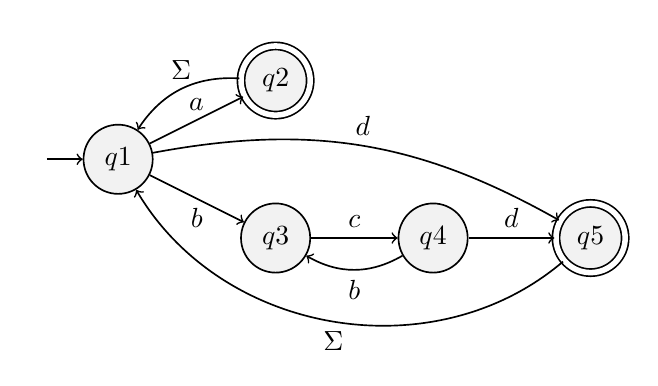
\begin{tikzpicture}
            \node[state, initial] (n1) {$q1$};
            \node[state, accepting, right of=n1] at (0, 1) (n2) {$q2$};
            \node[state, right of=n1] at (0, -1) (n3) {$q3$};
            \node[state, right of=n3] (n4) {$q4$};
            \node[state, accepting, right of=n4] (n5) {$q5$};
            
            \draw   (n1) edge[above] node{$a$} (n2)
                    (n2) edge[bend right, above] node{$\Sigma$} (n1)
                    (n1) edge[below] node{$b$} (n3)
                    (n1) edge[bend left=20, above] node{$d$} (n5)
                    (n3) edge[above] node{$c$} (n4)
                    (n4) edge[bend left, below] node{$b$} (n3)
                    (n4) edge[above] node{$d$} (n5)
                    (n5) edge[bend left=50, below] node{$\Sigma$} (n1);
        \end{tikzpicture}
        
        \item ((0\verb | 1)*(2\verb | 3)+)\verb | 0011 \\
        
        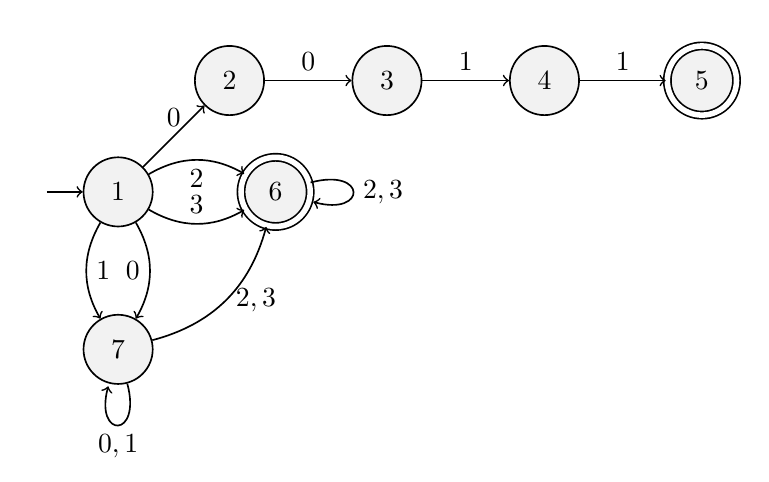
\begin{tikzpicture}
            \node[state, initial] (n1) {$1$};
            \node[state, above right of=n1] (n2) {$2$};
            \node[state, right of=n2] (n3) {$3$};
            \node[state, right of=n3] (n4) {$4$};
            \node[state, accepting, right of=n4] (n5) {$5$};
            \node[state, accepting, right of=n1] (n6) {$6$};
            \node[state, below of=n1] (n7) {$7$};
            
            \draw   (n1) edge[above] node{$0$} (n2)
                    (n2) edge[above] node{$0$} (n3)
                    (n3) edge[above] node{$1$} (n4)
                    (n4) edge[above] node{$1$} (n5)
                    (n1) edge[bend left, left] node{$0$} (n7)
                    (n1) edge[bend right, right] node{$1$} (n7)
                    (n1) edge[bend left, below] node{$2$} (n6)
                    (n1) edge[bend right, above] node{$3$} (n6)
                    (n7) edge[loop below, below] node{$0,1$} (n7)
                    (n7) edge[bend right, right] node{$2,3$} (n6)
                    (n6) edge[loop right, right] node{$2,3$} (n6);
        \end{tikzpicture}
        
        \item (a NOT(a))*aaa \\
        
        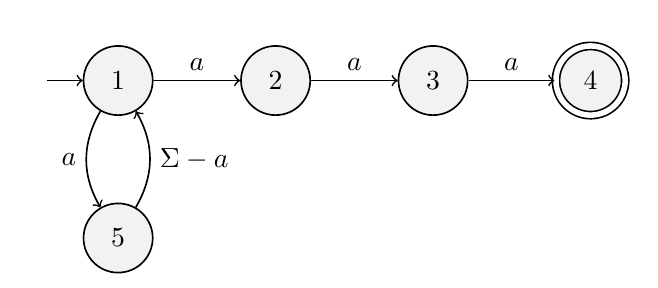
\begin{tikzpicture}
            \node[state, initial] (n1) {$1$};
            \node[state, right of=n1] (n2) {$2$};
            \node[state, right of=n2] (n3) {$3$};
            \node[state, accepting, right of=n3] (n4) {$4$};
            \node[state, below of=n1] (n5) {$5$};
            
            \draw   (n1) edge[above] node{$a$} (n2)
                    (n2) edge[above] node{$a$} (n3)
                    (n3) edge[above] node{$a$} (n4)
                    (n1) edge[bend right, left] node{$a$} (n5)
                    (n5) edge[bend right, right] node{$\Sigma-{a}$} (n1);
        \end{tikzpicture}
        
    \end{enumerate}
    
    
\end{enumerate}

\subsection{\textit{Dragon}}

\begin{enumerate}

    \item 3.3.4
    
    To write the regex for a keyword in a case insensitive language, you need to include both the lower and uppercase characters for any character used in a keyword. As an example, I have written how Select would look in a case insensitive language: [sS][eE][lL][eE][cC][tT].
    
\end{enumerate}

\end{document}